\section{Results and Discussion}\label{sec:results}
\subsection{Data Quality and Experimental Outcomes}
The processed dataset contains 20 participants, with ten in each assigned group; the exported quality summary reports no duplicate, missing, or invalid processed records. Table~\ref{tab:memory} presents group means and MAP--TBT differences for the two pre-specified outcomes. Group standard deviations were 17.51 (MAP) and 13.98 (TBT) percentage points for direction recall, and 8.50 and 11.60 points, respectively, for landmark recognition. These descriptive spreads emphasize that a difference in sample means is not, by itself, proof of a stable population effect.

\begin{table}[t]
\caption{Memory Outcomes: Group Means and MAP--TBT Differences}\label{tab:memory}
\centering\footnotesize
\begin{tabular}{lrrrl}\toprule
Outcome & MAP & TBT & $\Delta$ & 95\% CI for $\Delta$\\\midrule
Direction recall & 78\% & 72\% & +6 pp & [$-6$, 20] pp\\
Landmark recognition & 85\% & 67\% & +18 pp & [10, 27] pp\\\bottomrule
\end{tabular}
\end{table}

As defined by Eq.~\ref{eq:accuracy} and Eq.~\ref{eq:delta}, MAP had a 6-percentage-point advantage in direction recall. Its 95\% bootstrap CI crossed zero, so these data do not clearly distinguish a positive effect from no difference or a modest negative effect. Landmark recognition favored MAP by 18 points; its bootstrap interval was entirely positive. Fig.~\ref{fig:diff} shows both contrasts with uncertainty intervals. The exact one-sided permutation tests yielded $p=0.2894$ for direction recall and $p=0.00065$ for landmark recognition. At $\alpha=0.05$, only the landmark result supports the revised directional alternative. These post-data tests should not be represented as prospectively specified confirmatory evidence. Because only ten participants were assigned to each group, interval stability and sensitivity to individual responses remain concerns.

\begin{figure}[t]
\centering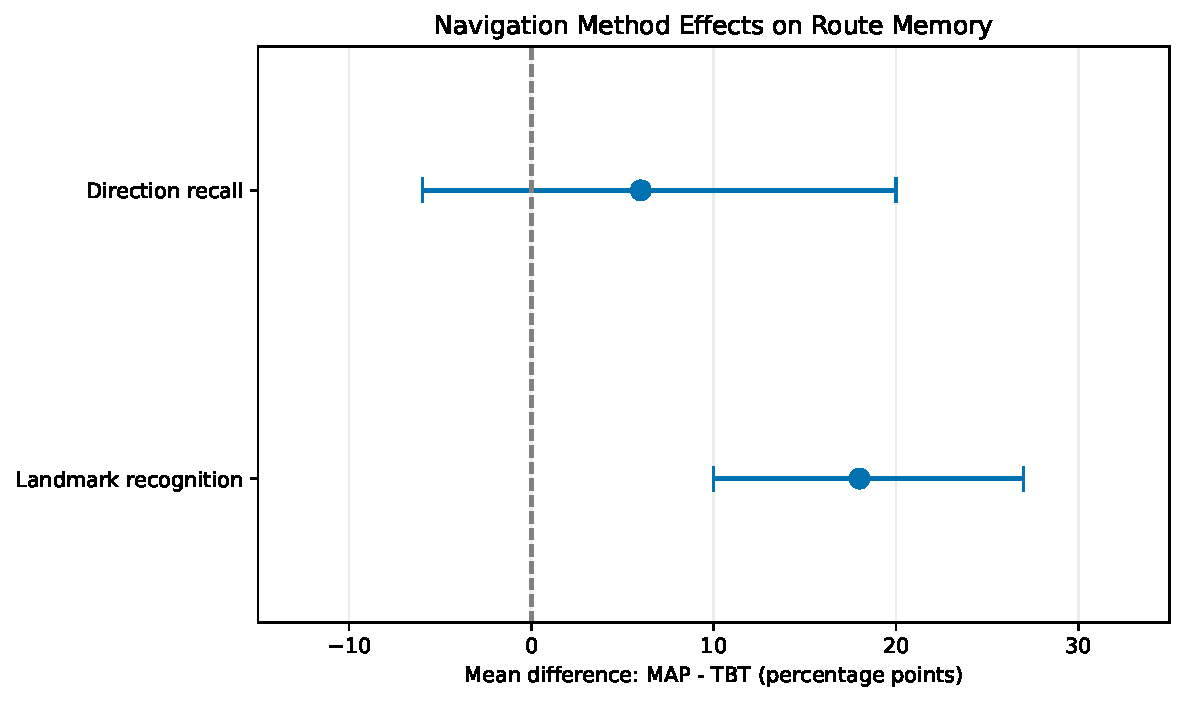
\includegraphics[width=0.98\columnwidth]{figures/group_differences.pdf}
\caption{MAP minus TBT mean accuracy (percentage points); percentile bootstrap 95\% CIs. The vertical zero line indicates no observed group difference.}\label{fig:diff}
\end{figure}

\subsection{Navigation Habits (RQ1)}
The questionnaire asked every participant about both methods rather than asking each experimental group about only its assigned treatment. Mean reported use was 15.65 TBT trips and 9.70 prior-map-study trips over the preceding 30 days, a paired difference of 5.95 trips (bootstrap 95\% CI: 2.30--9.60). Fig.~\ref{fig:habits} summarizes this descriptive comparison. Habit frequency cannot establish that one navigation method causes better memory, nor should the paired habit contrast be confused with the randomized MAP--TBT accuracy comparison.
\begin{figure}[t]
\centering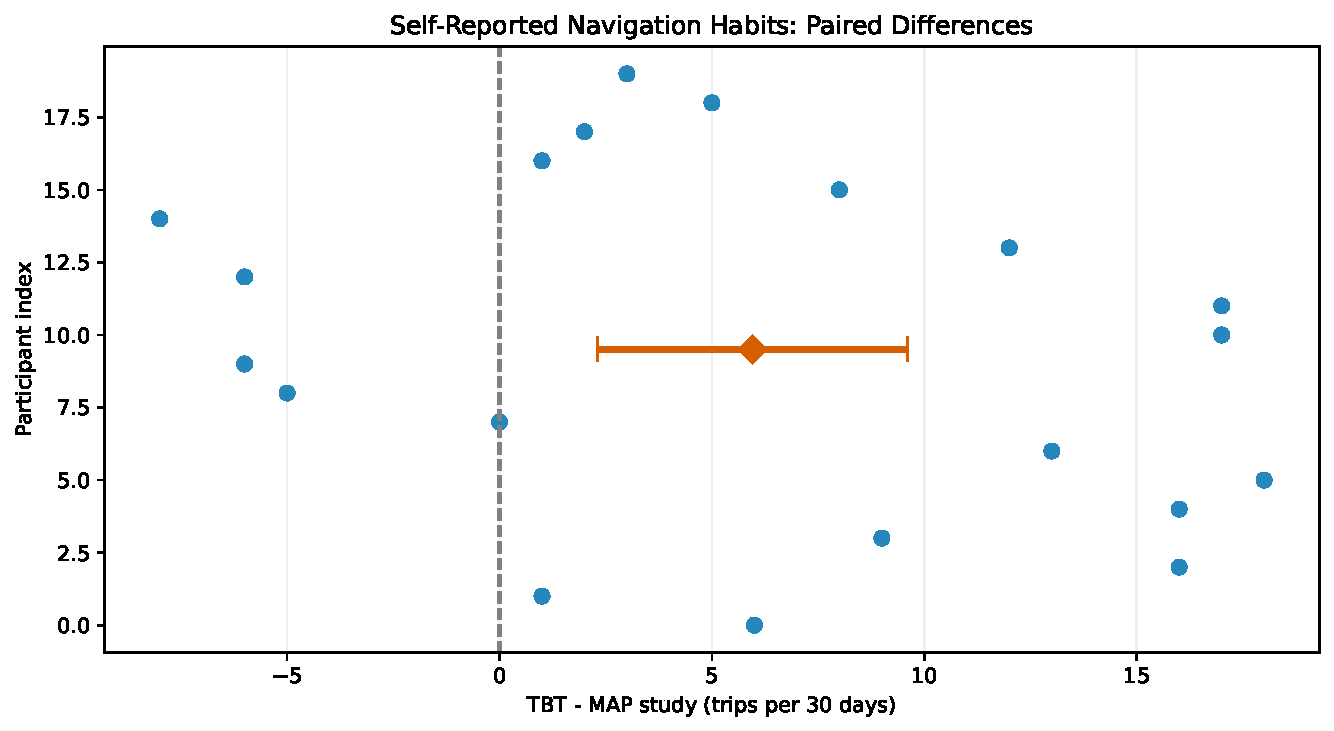
\includegraphics[width=0.95\columnwidth]{figures/navigation_habits.pdf}
\caption{Self-reported use of TBT and prior map study for unfamiliar routes in the preceding 30 days (paired responses, $N=20$).}\label{fig:habits}
\end{figure}

\subsection{Interpretation in Relation to Prior Work}
The observed direction of both contrasts is consistent with the theory-motivated expectation that advance map exposure may promote active encoding of route features. The stronger landmark result is compatible with evidence that maps and configural information can aid some forms of spatial learning~\cite{meneghetti_navigating_2021,munzer_navigation_2012}. Nevertheless, the earlier virtual-environment study found no advantage on route retracing, illustrating why the present direction and landmark outcomes should not be treated as interchangeable~\cite{meneghetti_navigating_2021}. Landmark-enriched TBT instructions can themselves promote incidental route learning~\cite{wunderlich_landmark_2023}; thus, TBT is not inherently incompatible with memory acquisition. The present experiment estimates a difference between two complete protocols, not a universal effect of all map interfaces versus all guided-navigation systems.

\subsection{What the Estimates Do and Do Not Show}
A useful distinction is between \emph{direction of the sample contrast}, \emph{precision}, and \emph{causal interpretation}. For both memory outcomes, the sample mean was higher under MAP. This is a descriptive fact about the 20 observations, not an automatic rejection of a null hypothesis. The exact one-sided test does not reject the direction-recall null, whereas it rejects the landmark-recognition null at the nominal 5\% threshold; the hypothesis revision after data collection limits confirmatory interpretation. The bootstrap interval for direction recall includes values below and above zero, indicating that the present sample does not reliably distinguish a modest MAP advantage from comparable performance. For landmarks, the entire estimated interval is positive. Nevertheless, the interval is conditional on the chosen participants, protocol, scoring rules, and resampling procedure; it does not cover uncertainty about whether a different route would produce the same pattern.

Direction choices and landmark recognition capture related but distinct forms of route memory; neither measures full survey knowledge~\cite{kim_landmark_2021}.

\subsection{Practical Interpretation}
The TBT condition is an active comparator: participants still received digital navigational support, and both conditions involved the same walking task. The comparison is therefore not MAP against no assistance. A practical implication is that previewing a route may be worth studying as a supplement to guidance when remembering environmental cues matters. This is a hypothesis for future application, not a demonstrated improvement in navigation safety, efficiency, or long-term retention. The current study did not measure walking time, navigation errors during traversal, or performance after days or weeks. A future factorial design could hold map content constant while independently varying advance preview and in-route prompts, clarifying whether timing, interface, or attention allocation explains the observed pattern.
